
\chapter{Cu-Substrate Recipe Optimization}
    
We attempted to optimize the recipe for Nb$_3$Sn fabrication on Cu substrates. We investigated the effect of the thickness and Sn concentration of the Cu-Sn film, %the type of diffusion barrier used
and the order of the Nb and Cu-Sn layers. We also experimented with hot-bronze, a post-reaction, and a hot bronze with a post-reaction while varying reaction times and temperatures. When the Nb$_3$Sn is reacted and forms at 700 $^{\circ}$C, the multilayer structure will cool down, and the Cu will thermally contract more than the Nb$_3$Sn. This leads to a large compressive strain in the Nb$_3$Sn film, much like was seen for the bronze substrate experiments. This can be mitigated using different growth modes with varying residual strain levels frozen into the lattice. For example, a different growth mode is present in hot bronze vs the post-reaction, leading to varying levels of residual strain in the film. The thin films underneath the Nb$_3$Sn film also affect the strain in the Nb$_3$Sn layer and can mitigate or exacerbate the already large strain due to the substrate thermal expansion.
    
    \section{Cu-Sn film Thickness and Sn\% Variation}

    We tested different Cu-Sn film thicknesses (2, 5, and 10 microns) with varying tin content (13\%, 24\%, 33\%, and 40\%) wt. on a 500-nanometer-thick Ta diffusion barrier. Three deposition with heat treatments were used: hot bronze, post-reaction, and hot bronze with post-reaction. We measured the $T_c$ for all films, and the critical temperature onset is given in \cref{tbl:2micronTc,tbl:5micronTconsettablecropped,tbl:10micronTconsetcropped}. Key magnetization curves and cross-sections are added for select films.


    \subsection{2 \si{\um} film}

    %change this should all be hot bronze....
    
    The $T_c$ onset for Nb$_3$Sn films on Cu substrates with 2 \si{\um} Cu-Sn layer are presented in Table \ref{tbl:2micronTc}. For the first and third heat treatments, we applied a 30-minute and 1 hr pre-heat treatment at 715 $^{\circ}$C, respectively, before the Nb deposition held at 715 $^{\circ}$C. This pre-heating did not affect the $T_c$ of the samples. For the second heat treatment, the sample had a 30 min pre-heating
    
    \begin{table}[h]
        \centering
                \caption[$T_c$ onset given for 2 µm thick Cu-Sn samples.]{$T_c$ onset given for 2 µm thick Cu-Sn samples. The first two samples with 40\% wt. Sn has two transitions with poor Tc around 12 K and 11 K and had unusual $T_c$ curves, possibly due to instrumentation error. They are denoted as question marks in the table.}
        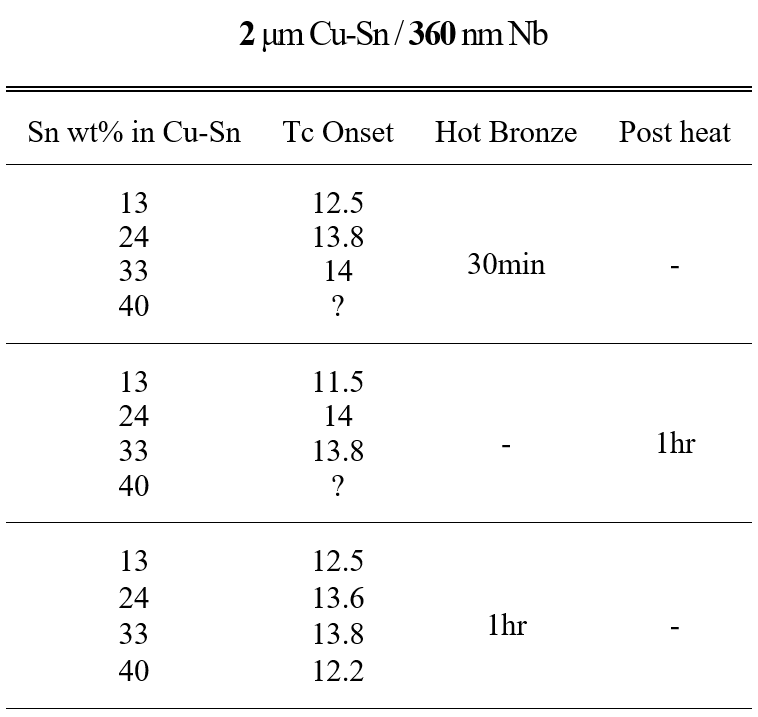
\includegraphics[width=.5\textwidth]{images/Cu/CuSnThickness/2micron Tc onset in table.png}

        \label{tbl:2micronTc}
    \end{table}
    
    
    The $T_c$ onset is low for films with this geometry because of the low Sn volume available for the Nb$_3$Sn reaction. The films had uniform thickness throughout. We found a peak critical temperature at 24\% and 33\% wt. Sn. This aligns with the work done on Nb substrates as seen in Figure \ref{fig:NbSubUpdated}.

    %Fig Sn concentration across layer
    %Fig cross section showing uniformty 
    
    \subsection{5 \si{\um} film}

    Copper substrates with a 5-micron Cu-Sn layer and varying Sn content: 13\%, 24\%, and 33\% deposited on a 500-nanometer-thick Ta layer were used. We then applied three different heat treatments (hot bronze, post-reaction, and hot bronze) in-situ with a 360-nanometer-thick Nb film. Full magnetization curves help show $\Delta$ Tc, which represents the volume fraction of high $T_c$ Nb$_3$Sn (assuming no screening).
    
    \begin{table}[h]
        \centering
                \caption[$T_c$ onset given for 5 µm thick Cu-Sn samples.]{$T_c$ onset given for 5 µm thick Cu-Sn samples.
        $^a$ Full magnetization curves of hot bronze recipes are shown in Fig. \ref{fig:5micronTc}.}
        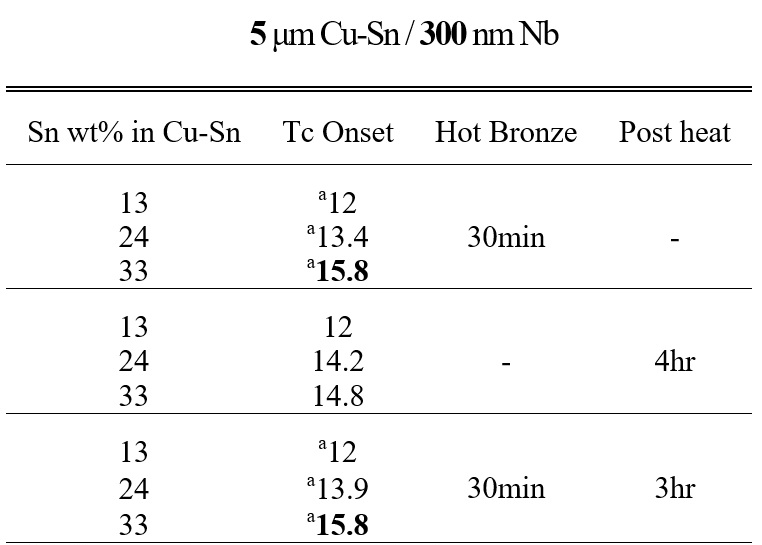
\includegraphics[width=.5\textwidth]{images/Cu/CuSnThickness/5micronTconsettablecropped.png}

        \label{tbl:5micronTconsettablecropped}
    \end{table}
    

    
    %and the films showed uniform thickness throughout, as seen in Fig(Show Figure.)
    
    \begin{figure}
        \centering
        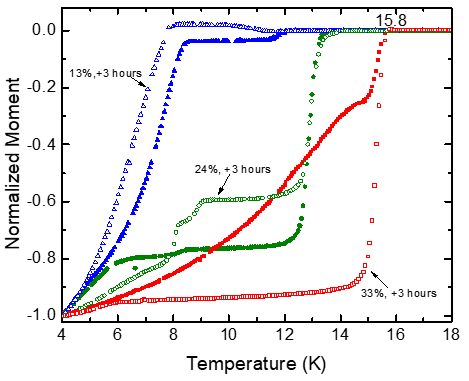
\includegraphics[width=.5\textwidth]{images/Cu/CuSnThickness/5micronTc.png}
        \caption{Magnetization curves for Cu Substrate films with select 5 µm Cu-Sn film obtained by the Hot bronze method (Recipe 1, filled symbols) with post-reaction (Recipe 3, open symbols).}
        \label{fig:5micronTc}
    \end{figure}
    

    The highest $T_c$ onset is $\approx$ 16K for the 33\% wt. Sn Cu-Sn film with a hot-bronze Nb deposition and a post-reaction. The post-reaction helped increase Sn concentration in the low Sn Nb$_3$Sn made during the hot-bronze reaction, as seen from Fig. \ref{fig:5micronTc} when comparing the two red curves. The $T_c$ onset may be misleading when looking at the full curves. The 24\% film seems to have two transitions, one at 12 and one at 14, not exemplified by just reading the $T_c$ onset. It is always necessary to analyze the full critical temperature curve and show details when necessary.
    
    %Sn concentration
    %Cu-Sn film look good? uniformity??
    
    \subsection{10 micron film}

    For the 10-micron experiment, copper substrates with a 10-micron Cu-Sn layer and varying Sn content: 24\% and 33\% deposited on a 500-nanometer-thick Ta layer were used. We then applied three different heat treatments (hot bronze, post-reaction, and hot bronze) in-situ with a 500-nanometer-thick Nb film. 
    
    \begin{table}[h]
        \centering
        \caption[$T_c$ onset given for 10 µm thick Cu-Sn samples.]{$T_c$ onset given for 10 µm thick Cu-Sn samples. $^a$ Heated to 680 $^{\circ}$C instead of usual 715 $^{\circ}$C. $^b$ Cross-section microstructure of film shown in Fig. \ref{fig:FullNb3Sn10micron}}
        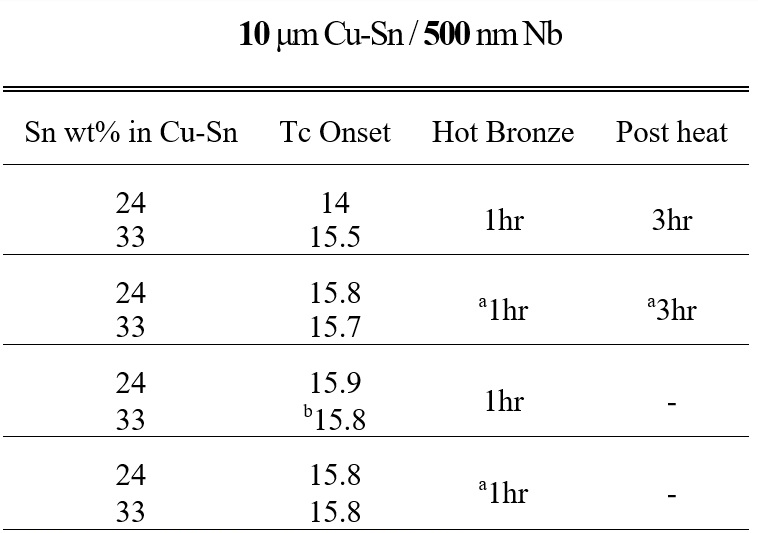
\includegraphics[width=.5\textwidth]{images/Cu/CuSnThickness/10micronTconsetcropped.png}
        \label{tbl:10micronTconsetcropped}
    \end{table}
    
    
    

    

    
    
    %Need roughness data to prove this. Add figure with 3d from optical of 10 micrometer film.
    
    
    Sn content and uniformity in the Nb$_3$Sn film can be evaluated using the SEM image and EDS line scan as seen in Fig. 2. This figure analyzes the microstructure of a sample that was made with recipe 1(the hot bronze technique) with a 10µm thick 33\%wt Sn Cu-Sn film and is described in table 1c. The microstructure of these films does not look like the cartoon in Fig. 2. There is a Cu-Sn layer that is discontinuous in three horizontal layers. The thin Nb$_3$Sn film that lies on top of the Cu-Sn film has uniform thickness, but its roughness is dependent on the underlying Cu-Sn film. As shown on the left side of Figure 2, a), the Cu-Sn film is non-uniform, and the Nb follows this uniformity. The optical micrograph in Figure \ref{fig:FullNb3Sn10micron} a) shows the the Cu-Sn film with two phases in gold and silver color. This only occurred in the high Sn Cu-Sn film recipes \>13\% wt Sn. This Cu-Sn phase can be resolved in the EDS map in Figure \ref{fig:FullNb3Sn10micron} c), looking at the top film of the Cu and Sn signals. A homogenous 25\% Sn was found through the thickness of the Nb$_3$Sn film. 
    %( DISCUSSION Due to either EDS limit resolution or lack of thermodynamic mixing ). 
    The Ta layer is uniform but did not stop the Sn from poisoning the Cu substrate, as seen at the bottom of the Sn EDS map in Figure \ref{fig:FullNb3Sn10micron} c).

    \begin{figure}
        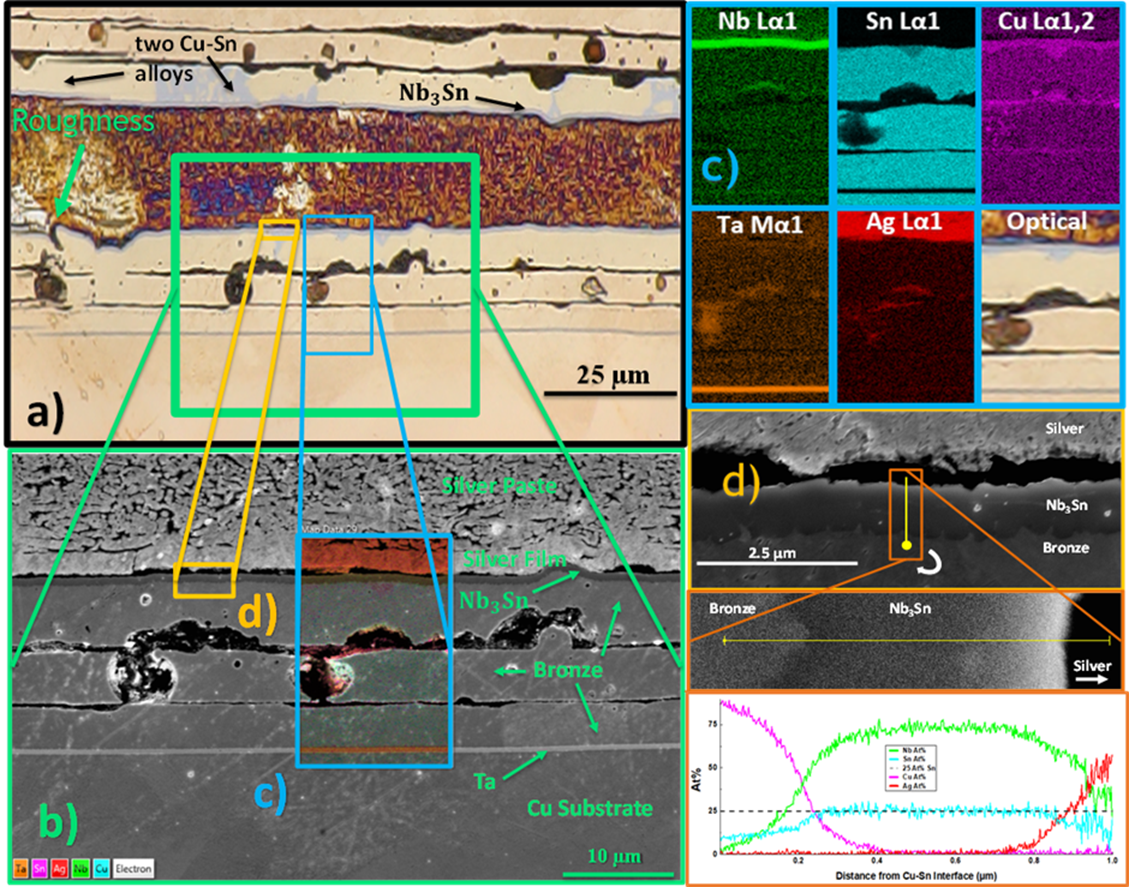
\includegraphics[width=\textwidth]{images/Cu/CuSnThickness/FullNb3Sn10micron.png}
        \caption[Images of bronze first film with EDS map and linescan.]{ Images of sandwiched Nb$_3$Sn film using optical microscope a) and SEM b). Blue insert c) shows the chemical composition of deposited and reacted layers using EDS mapping and an optical micrograph for comparison. The orange insert d) zooms into the 750nm Nb$_3$Sn film and measures the ideal 25 \% at. Sn throughout the thickness of our film. }
        \label{fig:FullNb3Sn10micron}
    \end{figure}
    
    
    %\subsection{Varying diffusion barriers (Ta, Nb, W)}

    %In this study, we chose Nb, Ta, and W as diffusion barriers and studied how well they acted for their intended purpose: as walls to stop Sn flow into the Cu substrate. These diffusion barriers can also help mitigate CTE mismatch and, therefore, reduce strain. We studied the microstructure and $T_c$ of these films. 

    
    
    %\paragraph{results}
    
    %Cross-sectional FIB SEM/EDS analysis is shown for with a Ta diffusion barrier in Figure \ref{fig:WenuraEDS}. There is void space in the middle of the Cu-Sn film, which is due to Sn diffusion out of the Cu-Sn film. There is little to no Sn below the Ta barrier, so the Ta layer successfully acted as a diffusion barrier. 
    
    %Nb, and W diffusion barrier. For the case of Ta and W, Sn seems not to pass the diffusion barrier and a large strain seems to build up that causes the Cu-Sn film to fracture and many voids to form. For the Nb diffusion barrier case, less Cu-Sn fracture was seen, and Sn seemed to be allowed through the Nb diffusion barrier even if the Nb diffusion barrier was not fully reacted.
    
    
    \begin{figure}
        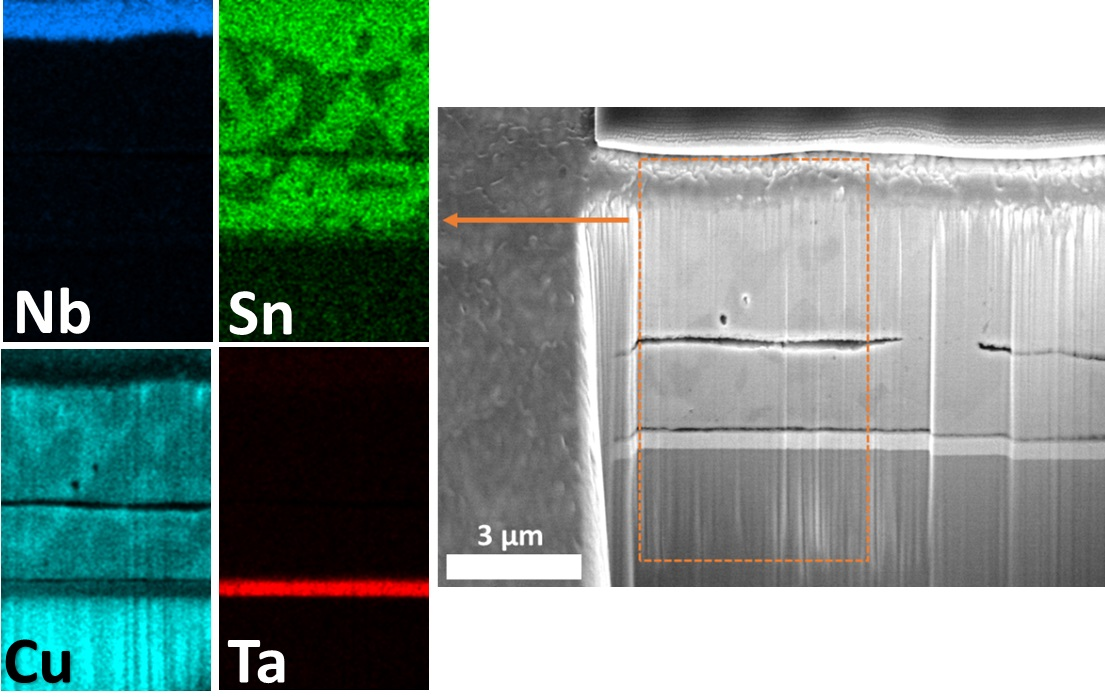
\includegraphics[width=\textwidth]{images/Cu/CuSnThickness/wenura EDS SEM.jpg}
        \caption{Sample 1: A Cu substrate with a 400nm Nb$_3$Sn film on 5µm of Cu - 33\% wt Sn and a 500nm thick Ta diffusion barrier. Characteristic void formation present in many bronze processes is found in the Cu-Sn layer, this might relieve strain on the Nb$_3$Sn leading to higher Tc.}
        \label{fig:WenuraEDS}
    \end{figure}

    %In Figure \ref{fig:2micron Nb3SnSEM}
    
    
    \begin{figure}
        \centering
        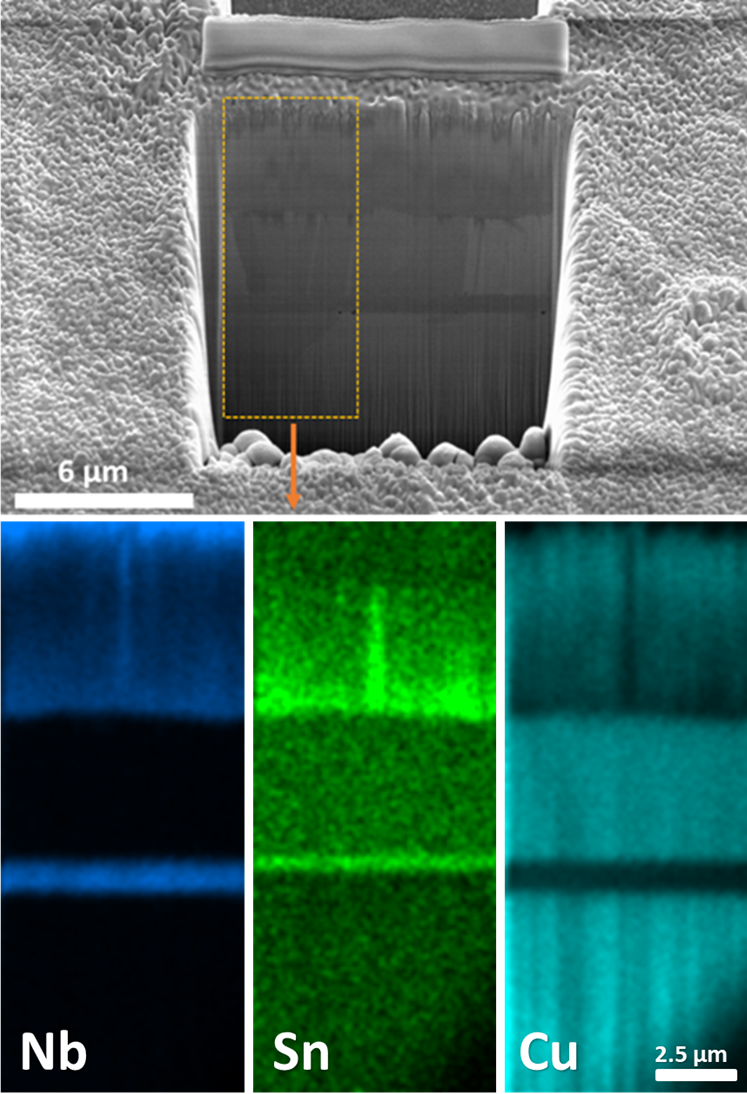
\includegraphics[width=.5\textwidth]{images/Cu/Diffusion/AS060823_38_Cu_EDS.png}
        \caption{Sample 2: A Cu substrate with a 2µm Nb$_3$Sn film on 4µm of Cu - 38\% wt Sn with a 500nm thick Nb diffusion barrier. Crack and void formation in the bronze layer was not found in this Nb diffusion barrier sample.}
        \label{fig:2micron Nb3SnSEM}
    \end{figure}

    %Fig 11. Show Figures where we can see Sn past W, Ta and not past Nb diffusion barrier. See cracking in Cu-SN film. 
    
    %Fig. 12 Show $T_c$ curves that compare the diffusion barriers.
    
    
    %\subsection{Discussion}
    
    %Give in dissertation
    